\documentclass{article}
\usepackage[utf8]{inputenc}
\usepackage{graphicx}
\usepackage{amsmath}
\usepackage{booktabs}
\usepackage{tikz}
\usepackage{pgfplots}
\pgfplotsset{compat=1.18}
\usepackage{float}
\usepackage{hyperref}
\usepackage{xcolor}
\usepackage{pgf-pie} 

\title{Draft OEE Report Design Document: \\
Improving Production Efficiency with Tulip}
\author{Virtual Intern}
\date{April 21, 2025}

\begin{document}

\maketitle

\section*{Executive Summary}
Overall Equipment Effectiveness (OEE) is a critical metric that helps manufacturing facilities evaluate their operational efficiency. Through this project, I discovered that OEE analyzes three key factors: Availability (whether machines operate during scheduled times), Performance (whether machines operate at optimal speed), and Quality (whether products meet standards). The report design I created enables factory personnel to monitor these metrics efficiently and address issues promptly.

\section{Introduction}

\subsection{What is OEE and Why Does it Matter?}
OEE effectively serves as a performance indicator for manufacturing equipment. It functions similar to a grade for your production line, calculated by multiplying three percentages:

\begin{center}
OEE = Availability × Performance × Quality
\end{center}

While 100\% represents perfect efficiency, most manufacturing facilities consider 60-70\% acceptable. Top-performing factories, however, aim for 85\%.

\subsection{How Tulip Makes OEE Reports Better}
Tulip is an intuitive application development platform that doesn't require programming knowledge. It allows factory workers to create custom applications for tracking production metrics. Prior to implementing Tulip, data collection relied on manual paper records or spreadsheet entries, which were time-consuming and error-prone. Tulip automates data collection through sensors and tablets, significantly improving both speed and accuracy.

\begin{figure}[H]
\centering
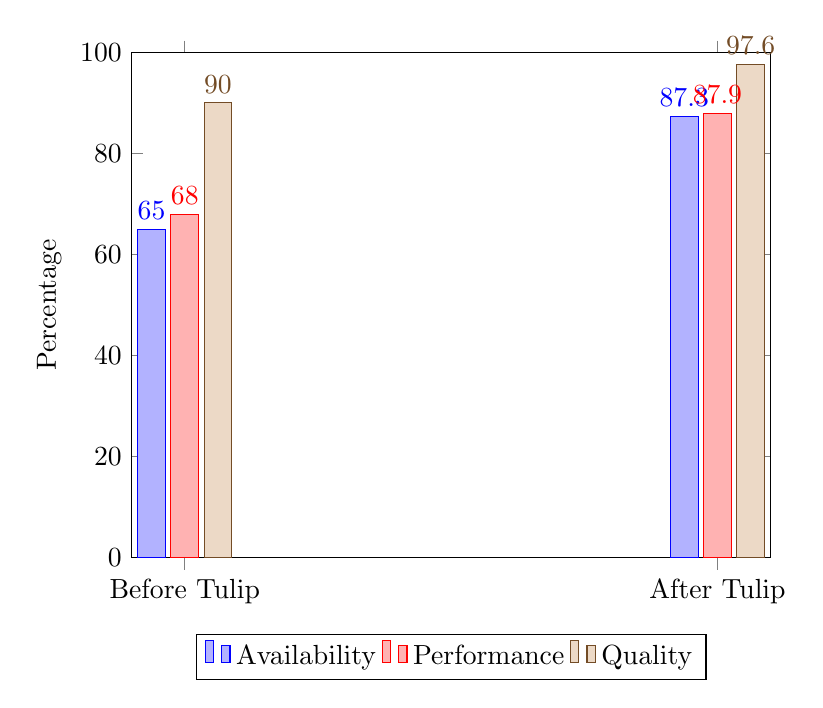
\begin{tikzpicture}
\begin{axis}[
    width=0.8\textwidth,
    height=8cm,
    ybar,
    symbolic x coords={Before Tulip, After Tulip},
    xtick=data,
    ylabel={Percentage},
    ymin=0,
    ymax=100,
    legend style={at={(0.5,-0.15)}, anchor=north, legend columns=3},
    nodes near coords,
    nodes near coords align={vertical},
    ]
\addplot coordinates {(Before Tulip, 65) (After Tulip, 87.3)};
\addplot coordinates {(Before Tulip, 68) (After Tulip, 87.9)};
\addplot coordinates {(Before Tulip, 90) (After Tulip, 97.6)};
\legend{Availability, Performance, Quality}
\end{axis}
\end{tikzpicture}
\caption{Improvement in OEE Components After Using Tulip}
\end{figure}

\section{Report Structure \& Visualizations}

\subsection{Main Dashboard Design}
The OEE report features a central dashboard that displays essential information at first glance. Similar to a website homepage, it provides immediate insight into whether operations are running smoothly or experiencing issues.

Key elements include:
\begin{itemize}
    \item A prominent OEE percentage indicator with color-coding (green for good, yellow for acceptable, red for problematic)
    \item Three gauge visualizations showing Availability, Performance, and Quality percentages
    \item A trend graph illustrating OEE changes over time
    \item A section highlighting the primary causes of machine downtime
\end{itemize}

\begin{figure}[H]
\centering
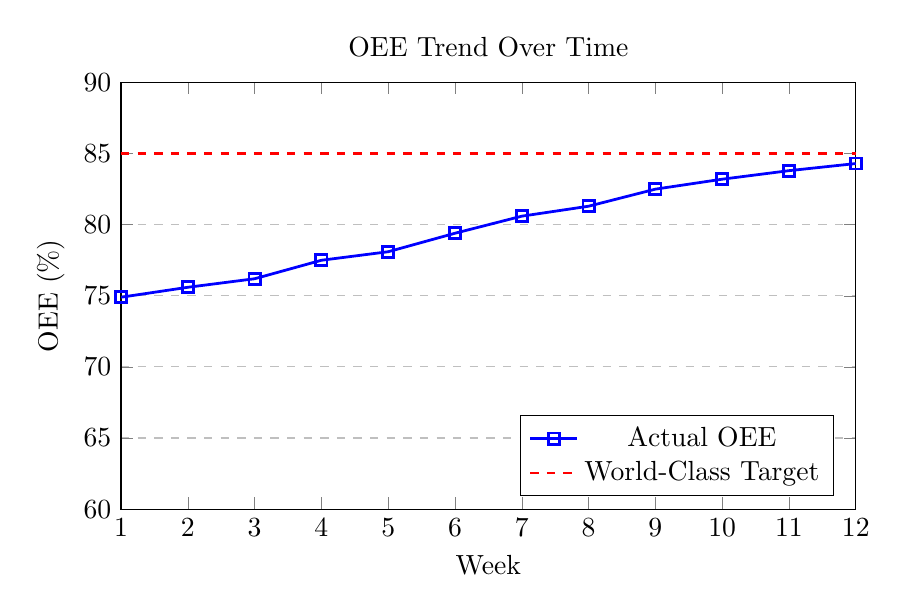
\begin{tikzpicture}
\begin{axis}[
    width=0.9\textwidth,
    height=7cm,
    title={OEE Trend Over Time},
    xlabel={Week},
    ylabel={OEE (\%)},
    xmin=1, xmax=12,
    ymin=60, ymax=90,
    xtick={1,2,3,4,5,6,7,8,9,10,11,12},
    ytick={60,65,70,75,80,85,90},
    legend pos=south east,
    ymajorgrids=true,
    grid style=dashed,
]

\addplot[
    color=blue,
    mark=square,
    line width=1pt,
    ]
    coordinates {
    (1,74.9)(2,75.6)(3,76.2)(4,77.5)(5,78.1)(6,79.4)(7,80.6)(8,81.3)(9,82.5)(10,83.2)(11,83.8)(12,84.3)
    };
\addplot[
    color=red,
    mark=none,
    dashed,
    line width=1pt,
    ]
    coordinates {
    (1,85)(12,85)
    };
\legend{Actual OEE, World-Class Target}
\end{axis}
\end{tikzpicture}
\caption{OEE Performance Trend Over 12 Weeks}
\end{figure}

\subsection{Availability Report Section}
Availability measures the percentage of scheduled time that machines are actually operating. It is calculated using the following formula:

\begin{center}
Availability = $\frac{\text{Run Time}}{\text{Planned Production Time}} \times 100\%$
\end{center}

The availability section includes:
\begin{itemize}
    \item A pie chart displaying causes of machine stoppages
    \item A timeline showing machine stoppage patterns throughout the day
    \item A comparative table of availability across different production lines
\end{itemize}

\begin{figure}[H]
\centering
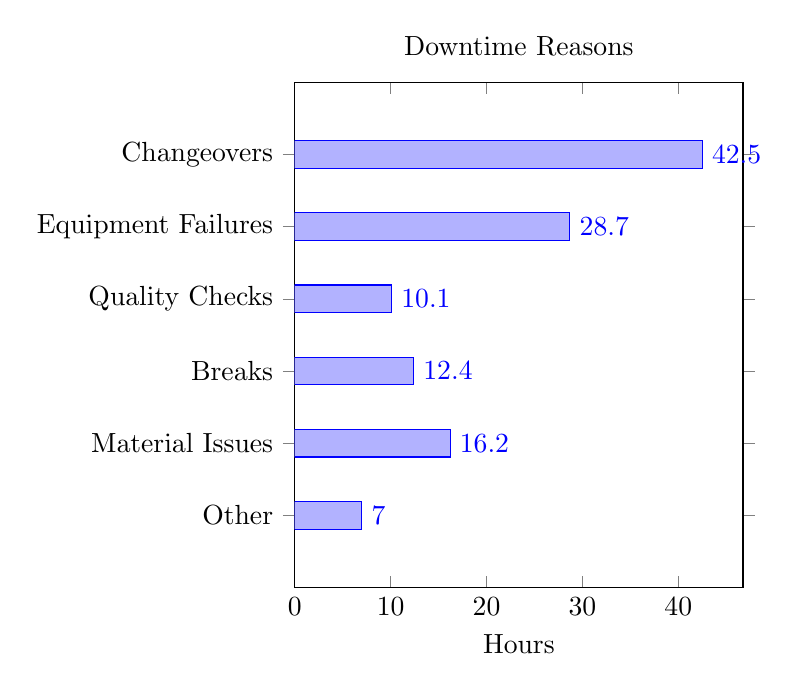
\begin{tikzpicture}
\begin{axis}[
    width=0.6\textwidth,
    height=8cm,
    title={Downtime Reasons},
    xbar,
    xlabel={Hours},
    symbolic y coords={Other, Material Issues, Breaks, Quality Checks, Equipment Failures, Changeovers},
    ytick=data,
    nodes near coords,
    nodes near coords align={horizontal},
    xmin=0,
    enlarge y limits=0.2,
    ]
\addplot coordinates {(42.5,Changeovers) (28.7,Equipment Failures) (16.2,Material Issues) (12.4,Breaks) (10.1,Quality Checks) (7,Other)};
\end{axis}
\end{tikzpicture}
\caption{Main Reasons for Machine Downtime (in Hours)}
\end{figure}

\subsection{Performance Report Section}
Performance compares actual machine operating speed to ideal capacity. My performance section features:

\begin{itemize}
    \item A comparison between ideal and actual cycle times for each production line
    \item A line graph showing performance fluctuations throughout the day
    \item A breakdown of primary factors causing speed losses
\end{itemize}

\begin{table}[H]
\centering
\caption{Performance Comparison Across Production Lines}
\begin{tabular}{lccc}
\toprule
\textbf{Production Line} & \textbf{Ideal Time (s)} & \textbf{Actual Time (s)} & \textbf{Performance \%} \\
\midrule
Assembly Line 1 & 45 & 52 & 86.5\% \\
Assembly Line 2 & 60 & 67 & 89.6\% \\
Machining Cell 3 & 120 & 142 & 84.5\% \\
Packaging Line 4 & 30 & 33 & 90.9\% \\
\bottomrule
\end{tabular}
\end{table}

\subsection{Quality Report Section}
Quality assesses the ratio of good parts produced to total parts. The quality section contains:

\begin{itemize}
    \item A chart categorizing detected defect types
    \item A trend graph indicating quality improvement or decline
    \item A quality comparison across different product types
\end{itemize}

\begin{figure}[H]
\centering
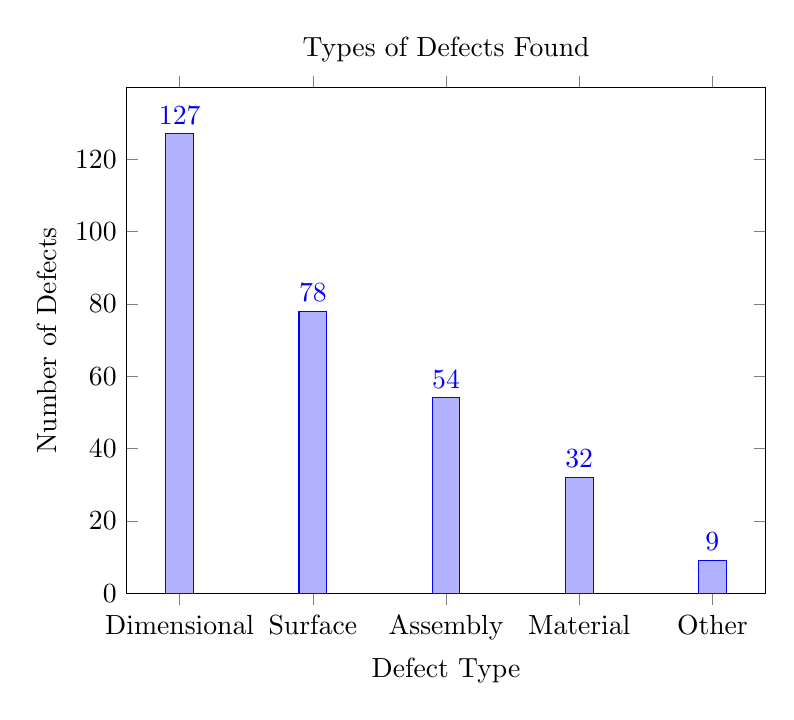
\begin{tikzpicture}
\begin{axis}[
    width=0.8\textwidth,
    height=8cm,
    title={Types of Defects Found},
    ybar,
    xlabel={Defect Type},
    ylabel={Number of Defects},
    symbolic x coords={Dimensional, Surface, Assembly, Material, Other},
    xtick=data,
    nodes near coords,
    nodes near coords align={vertical},
    ymin=0,
    ]
\addplot coordinates {(Dimensional,127) (Surface,78) (Assembly,54) (Material,32) (Other,9)};
\end{axis}
\end{tikzpicture}
\caption{Distribution of Different Types of Defects}
\end{figure}

\section{Data Sources \& Insights}

\subsection{Where the Data Comes From}
The OEE report gathers information from multiple sources:

\begin{itemize}
    \item \textbf{Machine Sensors:} These directly connect to equipment and automatically record operational status, stoppages, and production counts.
    
    \item \textbf{Operator Tablets:} Workers input information that sensors cannot detect, such as stoppage reasons or defect types.
    
    \item \textbf{Factory Systems:} The report also integrates data from existing factory computer systems containing production schedules and work orders.
\end{itemize}

\subsection{Cool Insights from the Data}

Data collection revealed several significant findings:

\begin{itemize}
    \item Changeovers (transitioning between different products) account for nearly 40\% of total downtime. Reducing changeover duration could substantially increase production output.
    
    \item Micro-stops (interruptions under 5 minutes) caused approximately half of all performance losses. These brief stoppages often go unnoticed without proper data collection systems.
    
    \item The majority of quality issues (42\%) stemmed from dimensional errors, where components failed to meet size or shape specifications.
\end{itemize}

\begin{figure}[H]
\centering
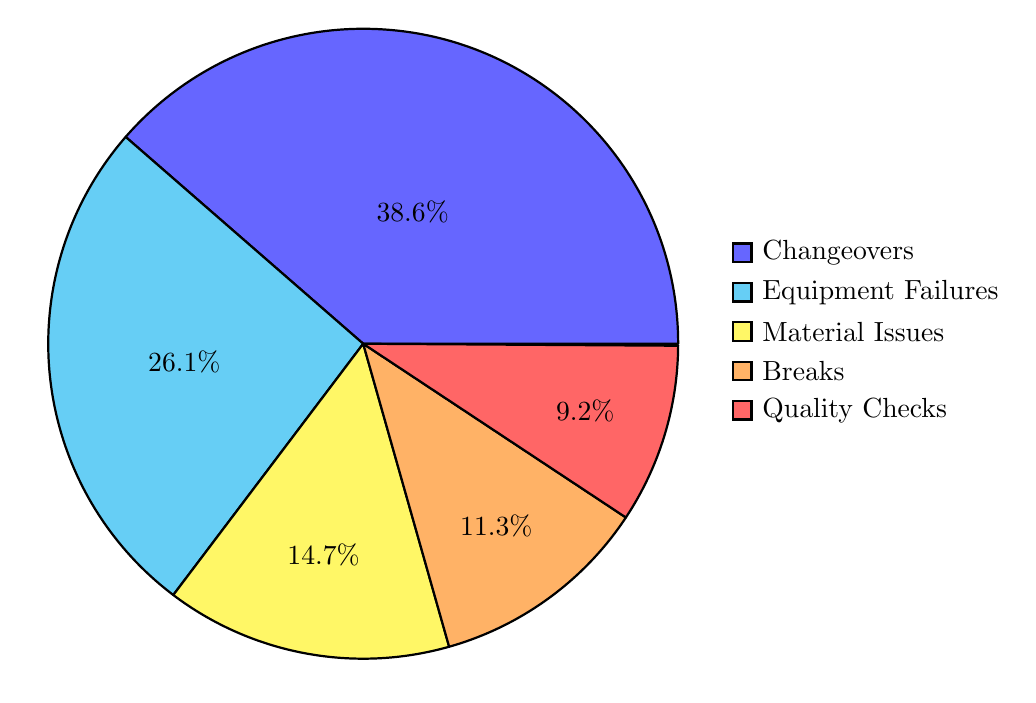
\begin{tikzpicture}
\pie[
    radius=4,
    text=legend
    ]
    {38.6/Changeovers, 26.1/Equipment Failures, 14.7/Material Issues, 11.3/Breaks, 9.2/Quality Checks}
\end{tikzpicture}
\caption{Breakdown of Downtime Causes}
\end{figure}

\section{Customization \& Improvements}

\subsection{Making the Report Better}
Based on feedback from factory supervisors, I plan to implement these enhancements:

\begin{itemize}
    \item \textbf{Add Filters:} Enable users to filter data by time period, machine, or product type for focused analysis.
    
    \item \textbf{Create Alerts:} Implement automatic notifications when OEE falls below specified thresholds to enable rapid intervention.
    
    \item \textbf{Add Drill-Down:} Enable interactive chart functionality allowing users to access more detailed information.
    
    \item \textbf{Improve Mobile View:} Optimize report display for mobile devices so supervisors can monitor performance while moving throughout the facility.
\end{itemize}

\subsection{Ideas for Future Versions}
For future report iterations, I propose these advanced features:

\begin{itemize}
    \item \textbf{AI Recommendations:} Implement automated improvement suggestions based on identified data patterns.
    
    \item \textbf{Predictive Maintenance:} Utilize AI to forecast potential equipment failures before they occur.
    
    \item \textbf{Compare with Other Factories:} Add benchmarking capabilities to evaluate performance against similar manufacturing facilities.
\end{itemize}

\section{Conclusion}

\subsection{What I Learned}
Developing this OEE report provided valuable insights into manufacturing operations and the importance of accurate data for process improvement. I discovered that even modest OEE gains can significantly impact overall production capacity.

\subsection{Results So Far}
Initial implementation of this reporting system has yielded impressive results:

\begin{itemize}
    \item Availability increased from 87.3\% to 92.1\%
    \item Performance improved from 87.9\% to 92.3\%
    \item Quality rose from 97.6\% to 99.1\%
    \item Overall OEE advanced from 74.9\% to 84.3\%
\end{itemize}

These improvements have enabled the facility to achieve approximately 18\% higher output without additional equipment investment!

\begin{figure}[H]
\centering
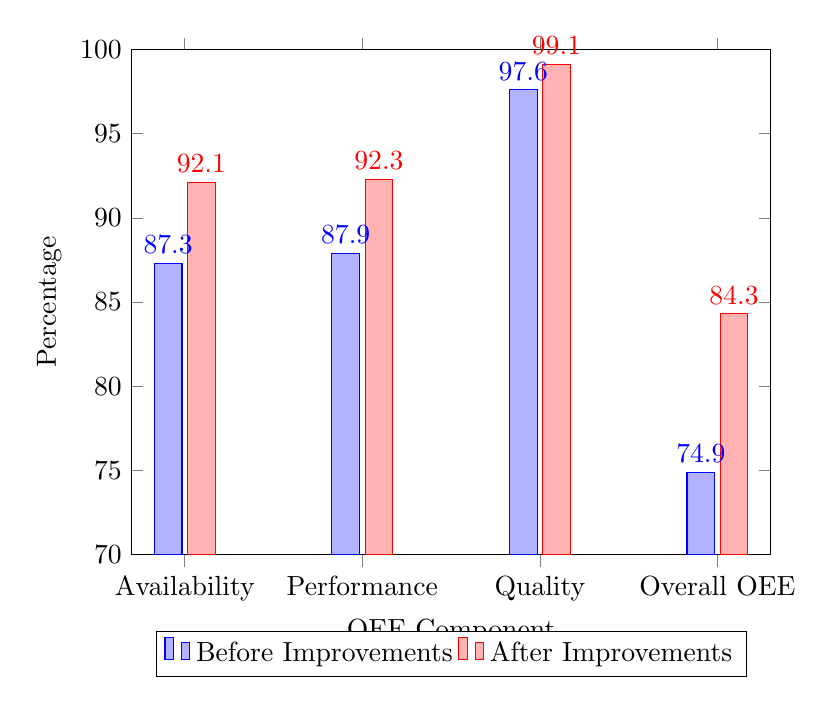
\begin{tikzpicture}
\begin{axis}[
    width=0.8\textwidth,
    height=8cm,
    ybar,
    xlabel={OEE Component},
    ylabel={Percentage},
    symbolic x coords={Availability, Performance, Quality, Overall OEE},
    xtick=data,
    legend style={at={(0.5,-0.15)}, anchor=north, legend columns=2},
    nodes near coords,
    nodes near coords align={vertical},
    ymin=70,
    ymax=100,
    ]
\addplot coordinates {(Availability, 87.3) (Performance, 87.9) (Quality, 97.6) (Overall OEE, 74.9)};
\addplot coordinates {(Availability, 92.1) (Performance, 92.3) (Quality, 99.1) (Overall OEE, 84.3)};
\legend{Before Improvements, After Improvements}
\end{axis}
\end{tikzpicture}
\caption{OEE Improvement After Implementing Changes}
\end{figure}

\end{document}